% Options for packages loaded elsewhere
\PassOptionsToPackage{unicode}{hyperref}
\PassOptionsToPackage{hyphens}{url}
%
\documentclass[
]{scrbook}
\usepackage{amsmath,amssymb}
\usepackage{iftex}
\ifPDFTeX
  \usepackage[T1]{fontenc}
  \usepackage[utf8]{inputenc}
  \usepackage{textcomp} % provide euro and other symbols
\else % if luatex or xetex
  \usepackage{unicode-math} % this also loads fontspec
  \defaultfontfeatures{Scale=MatchLowercase}
  \defaultfontfeatures[\rmfamily]{Ligatures=TeX,Scale=1}
\fi
\usepackage{lmodern}
\ifPDFTeX\else
  % xetex/luatex font selection
\fi
% Use upquote if available, for straight quotes in verbatim environments
\IfFileExists{upquote.sty}{\usepackage{upquote}}{}
\IfFileExists{microtype.sty}{% use microtype if available
  \usepackage[]{microtype}
  \UseMicrotypeSet[protrusion]{basicmath} % disable protrusion for tt fonts
}{}
\makeatletter
\@ifundefined{KOMAClassName}{% if non-KOMA class
  \IfFileExists{parskip.sty}{%
    \usepackage{parskip}
  }{% else
    \setlength{\parindent}{0pt}
    \setlength{\parskip}{6pt plus 2pt minus 1pt}}
}{% if KOMA class
  \KOMAoptions{parskip=half}}
\makeatother
\usepackage{xcolor}
\usepackage{longtable,booktabs,array}
\usepackage{calc} % for calculating minipage widths
% Correct order of tables after \paragraph or \subparagraph
\usepackage{etoolbox}
\makeatletter
\patchcmd\longtable{\par}{\if@noskipsec\mbox{}\fi\par}{}{}
\makeatother
% Allow footnotes in longtable head/foot
\IfFileExists{footnotehyper.sty}{\usepackage{footnotehyper}}{\usepackage{footnote}}
\makesavenoteenv{longtable}
\usepackage{graphicx}
\makeatletter
\def\maxwidth{\ifdim\Gin@nat@width>\linewidth\linewidth\else\Gin@nat@width\fi}
\def\maxheight{\ifdim\Gin@nat@height>\textheight\textheight\else\Gin@nat@height\fi}
\makeatother
% Scale images if necessary, so that they will not overflow the page
% margins by default, and it is still possible to overwrite the defaults
% using explicit options in \includegraphics[width, height, ...]{}
\setkeys{Gin}{width=\maxwidth,height=\maxheight,keepaspectratio}
% Set default figure placement to htbp
\makeatletter
\def\fps@figure{htbp}
\makeatother
\setlength{\emergencystretch}{3em} % prevent overfull lines
\providecommand{\tightlist}{%
  \setlength{\itemsep}{0pt}\setlength{\parskip}{0pt}}
\setcounter{secnumdepth}{5}
% definitions for citeproc citations
\NewDocumentCommand\citeproctext{}{}
\NewDocumentCommand\citeproc{mm}{%
  \begingroup\def\citeproctext{#2}\cite{#1}\endgroup}
\makeatletter
 % allow citations to break across lines
 \let\@cite@ofmt\@firstofone
 % avoid brackets around text for \cite:
 \def\@biblabel#1{}
 \def\@cite#1#2{{#1\if@tempswa , #2\fi}}
\makeatother
\newlength{\cslhangindent}
\setlength{\cslhangindent}{1.5em}
\newlength{\csllabelwidth}
\setlength{\csllabelwidth}{3em}
\newenvironment{CSLReferences}[2] % #1 hanging-indent, #2 entry-spacing
 {\begin{list}{}{%
  \setlength{\itemindent}{0pt}
  \setlength{\leftmargin}{0pt}
  \setlength{\parsep}{0pt}
  % turn on hanging indent if param 1 is 1
  \ifodd #1
   \setlength{\leftmargin}{\cslhangindent}
   \setlength{\itemindent}{-1\cslhangindent}
  \fi
  % set entry spacing
  \setlength{\itemsep}{#2\baselineskip}}}
 {\end{list}}
\usepackage{calc}
\newcommand{\CSLBlock}[1]{\hfill\break\parbox[t]{\linewidth}{\strut\ignorespaces#1\strut}}
\newcommand{\CSLLeftMargin}[1]{\parbox[t]{\csllabelwidth}{\strut#1\strut}}
\newcommand{\CSLRightInline}[1]{\parbox[t]{\linewidth - \csllabelwidth}{\strut#1\strut}}
\newcommand{\CSLIndent}[1]{\hspace{\cslhangindent}#1}
\usepackage{booktabs} % for better tables

% fonts
% libertine font: https://www.tug.org/FontCatalogue/linuxlibertine/
\usepackage[oldstyle]{libertine}
\usepackage{libertinust1math}
% \usepackage[T1]{fontenc}
\usepackage[extralight]{inter} 

\usepackage[left=3cm, right=2.5cm, top=2.5cm, bottom=4cm]{geometry} % page margings

\usepackage{tabto} % for aligning text at a certain position, used for title page

\usepackage[ngerman, english]{babel}		% main language is the last in the list, more infor is here: https://en.wikibooks.org/wiki/LaTeX/Internationalization#Babel

\usepackage[onehalfspacing]{setspace}	% clean 1.5 leading / spacing
\RedeclareSectionCommand[beforeskip=0.5em,afterskip=2em]{chapter} % define space before and after heading

\usepackage{pdfpages} % to include pdfs
\ifLuaTeX
  \usepackage{selnolig}  % disable illegal ligatures
\fi
\usepackage{bookmark}
\IfFileExists{xurl.sty}{\usepackage{xurl}}{} % add URL line breaks if available
\urlstyle{same}
\hypersetup{
  hidelinks,
  pdfcreator={LaTeX via pandoc}}

\author{}
\date{\vspace{-2.5em}}

\begin{document}

\frontmatter

\begin{titlepage}                   
    \begin{center}
        
\includegraphics[height=3.2cm]{logo.pdf}\\[40mm]
        
        \huge {\linespread{1.5} Rethinking Variation in Social Cognition: \\ Gaze Following across Individuals, Ages, and Communities}\\[30mm]
        
                
        \normalsize Von der Fakultät Nachhaltigkeit \\ der Leuphana Universität Lüneburg zur Erlangung des Grades\\
        Doktorin der Psychologie\\-- Dr. rer. nat. --\\[10mm]
        
        genehmigte Dissertation von\\[10mm]
        Julia Christin Prein\\
        geboren am TT.MM.JJJJ in XXX
        
    \vspace*{\fill} 
    \end{center}
    
    \newpage
    \thispagestyle{empty}
    \begin{flushleft}
      \begin{normalsize}
      
      \vspace*{\fill} 
            Eingereicht am: \tabto*{30mm} 1. Oktober 2024 \\[10mm]
            
            Erstbetreuer: \tabto*{30mm} Prof.\,Dr.\, Manuel Bohn, \textit{Leuphana Universität Lüneburg}\\
                Zweitbetreuer: \tabto*{30mm} Prof.\,Dr.\, Sebastian Wallot, \textit{Leuphana Universität Lüneburg}\\[10mm]
                
                Erstgutachter: \tabto*{30mm} Prof.\,Dr.\, Manuel Bohn, \textit{Leuphana Universität Lüneburg}\\
                Zweitgutachter: \tabto*{30mm} Prof.\,Dr.\, Sebastian Wallot, \textit{Leuphana Universität Lüneburg}\\
                Drittgutachter: \tabto*{30mm} Prof.\,Dr.\, Daniel Haun, \textit{Universität Leipzig \& Max-Planck-Institut für\\
                \tabto*{30mm} Evolutionäre Anthropologie}\\[10mm]
        \end{normalsize}
    \end{flushleft}
    
\end{titlepage}

\tableofcontents

\chapter{Copyright Notice}\label{copyright}

The research articles included in this cumulative dissertation have been or will be published in international peer-reviewed journals. Copyright of the text and illustrations lies with the author or authors of the respective chapter(s). The publishers own the exclusive rights to publish or use the text and illustrations for their own purposes. Reprinting any part of this dissertation thesis requires the permission of the copyright holder(s).
The individual contributions of this cumulative thesis have been or will be published (in chronological order) as follows:

Prein, J. C., Kalinke, S., Haun, D. B. M.*, \& Bohn, M.* (2023). TANGO: A reliable, open-source, browser-based task to assess individual differences in gaze understanding in 3 to 5-year-old children and adults. \emph{Behavior Research Methods, 56}(3), 2469--2485. \url{https://doi.org/10.3758/s13428-023-02159-5}

Prein, J. C., Maurits, L., Werwach, A., Haun, D. B. M.,* \& Bohn, M.* (2024). \emph{Variation in gaze understanding across the life span: A process-level perspective.} PsyArXiv. \url{https://doi.org/10.31234/osf.io/dy73a}

Bohn, M.*, Prein, J. C.*, Ayikoru, A., Bednarski, F. M., Dzabatou, A., Frank, M. C., Henderson, A. M. E., Isabella, J., Kalbitz, J., Kanngiesser, P., Keşşafoğlu, D., Koymen, B., Manrique-Hernandez, M., Magazi, S., Mújica-Manrique, L., Ohlendorf, J., Olaoba, D., Pieters, W., Pope-Caldwell, S., \ldots{} Haun, D. (2024). \emph{A universal of human social cognition: Children from 17 communities process gaze in similar ways.} PsyArXiv. \url{https://doi.org/10.31234/osf.io/z3ahv}

Prein, J.C., Bednarski, F. M., Dzabatou, A., Frank, M. C., Henderson, A. M. E., Kalbitz, J., Kanngiesser, P., Keşşafoğlu, D., Köymen, B., Manrique-Hernandez, M. V., Magazi, S., Mújica-Manrique, L., Ohlendorf, J., Olaoba, D., Pieters, W. R., Pope-Caldwell, S., Sen, U., Slocombe, K., Sparks, R. Z., Stengelin, R., Sunderarajan, J., Sutherland, K., Tusiime, F., Vieira, W., Zhang, Z., Zong, Y., Haun, D. B. M.*, Bohn, M.*. (2024). \emph{Measuring variation in gaze following across communities, ages, and individuals -- a showcase of the TANGO--CC.} PsyArxiv.

~

Further articles that were written in the context of this dissertation can be found in the Appendix and have been or will be published as follows (in chronological order):

Schuwerk, T., Kampis, D., Baillargeon, R., Biro, S., Bohn, M., Byers-Heinlein, K., Dörrenberg, S., Fisher, C., Franchin, L., Fulcher, T., Garbisch, I., Geraci, A., Grosse Wiesmann, C., Hamlin, K., Haun, D. B. M., Hepach, R., Hunnius, S., Hyde, D. C., Karman, P., \ldots, Prein, J., \ldots{} Rakoczy, H. (2021). \emph{Action anticipation based on an agent's epistemic state in toddlers and adults. Child Development} (In-Principle Acceptance of Registered Report Stage 1: Study Design). PsyArXiv. \url{https://doi.org/10.31234/osf.io/x4jbm}

Bohn, M., Prein, J. C., Engicht, J., Haun, D., Gagarina, N., \& Koch, T. (2023). \emph{PREVIC: An adaptive parent report measure of expressive vocabulary in children between 3 and 8 years of age.} PsyArXiv. \url{https://doi.org/10.31234/osf.io/hvncp}

Bohn, M.*, Prein, J.*, Koch, T., Bee, R. M., Delikaya, B., Haun, D., \& Gagarina, N. (2024). oREV: An item response theory-based open receptive vocabulary task for 3- to 8-year-old children. \emph{Behavior Research Methods, 56}(3), 2595--2605. \url{https://doi.org/10.3758/s13428-023-02169-3}

Steffan, A., Zimmer, L., Arias-Trejo, N., Bohn, M., Dal Ben, R., Flores-Coronado, M. A., Franchin, L., Garbisch, I., Grosse Wiesmann, C., Hamlin, J. K., Havron, N., Hay, J. F., Hermansen, T. K., Jakobsen, K. V., Kalinke, S., Ko, E.-S., Kulke, L., Mayor, J., Meristo, M., \ldots, Prein, J., \ldots, Schuwerk, T. (2024). Validation of an open source, remote web-based eye-tracking method (WebGazer) for research in early childhood. \emph{Infancy, 29}(1), 31--55. \url{https://doi.org/10.1111/infa.12564}

~

* denotes shared first or last authorship.

\chapter{Abstract}\label{abstract}

Prein et al. (\citeproc{ref-prein2023tango}{2023})

Lorem ipsum dolor sit amet, consectetur adipiscing elit, sed do eiusmod tempor incididunt ut labore et dolore magna aliqua. Luctus venenatis lectus magna fringilla urna. Laoreet non curabitur gravida arcu ac tortor. Faucibus vitae aliquet nec ullamcorper sit amet risus nullam eget. Cras semper auctor neque vitae tempus quam pellentesque. Imperdiet massa tincidunt nunc pulvinar sapien et ligula ullamcorper. Et tortor at risus viverra adipiscing at. Congue nisi vitae suscipit tellus mauris. Habitant morbi tristique senectus et netus et malesuada fames ac. Eget mauris pharetra et ultrices neque. Aenean et tortor at risus viverra. Tempor orci dapibus ultrices in iaculis nunc sed augue. Euismod lacinia at quis risus sed vulputate odio ut enim. Id eu nisl nunc mi ipsum faucibus. Est lorem ipsum dolor sit amet. Eget velit aliquet sagittis id consectetur purus. Faucibus ornare suspendisse sed nisi. Pellentesque diam volutpat commodo sed egestas egestas fringilla.

\chapter{Zusammenfassung}\label{zusammenfassung}

Lorem ipsum dolor sit amet, consectetur adipiscing elit, sed do eiusmod tempor incididunt ut labore et dolore magna aliqua. Luctus venenatis lectus magna fringilla urna. Laoreet non curabitur gravida arcu ac tortor. Faucibus vitae aliquet nec ullamcorper sit amet risus nullam eget. Cras semper auctor neque vitae tempus quam pellentesque. Imperdiet massa tincidunt nunc pulvinar sapien et ligula ullamcorper. Et tortor at risus viverra adipiscing at. Congue nisi vitae suscipit tellus mauris. Habitant morbi tristique senectus et netus et malesuada fames ac. Eget mauris pharetra et ultrices neque. Aenean et tortor at risus viverra. Tempor orci dapibus ultrices in iaculis nunc sed augue. Euismod lacinia at quis risus sed vulputate odio ut enim. Id eu nisl nunc mi ipsum faucibus. Est lorem ipsum dolor sit amet. Eget velit aliquet sagittis id consectetur purus. Faucibus ornare suspendisse sed nisi. Pellentesque diam volutpat commodo sed egestas egestas fringilla.

\chapter{Danksagung}\label{danksagung}

\mainmatter

\chapter{Introduction}\label{introduction}

\begin{itemize}
\tightlist
\item
  what makes use human?
\item
  social interactions \& communication
\item
  how does that develop?
\end{itemize}

\section{Social Cognition}\label{social-cognition}

\subsection{What}\label{what}

\begin{itemize}
\tightlist
\item
  Definitions of Social Cognition: not that clear\ldots{}
\item
  Quesque et al. (\citeproc{ref-quesque2024defining}{2024})
\item
  Expert survey: present results and quick methods, but not in detail
\end{itemize}

\section{Gaze Following}\label{gaze-following}

\subsection{What}\label{what-1}

\begin{itemize}
\tightlist
\item
  maybe: how relates to joint attention
  \#\#\# Why important
\item
  action coordination
\item
  common ground =\textgreater{} word learning
\item
  gafo predicts real-life outcomes (language, school performance)
\item
  open questions: Gustaf paper
\end{itemize}

\section{Individual Differences}\label{individual-differences}

\subsection{What}\label{what-2}

\subsection{Why}\label{why}

\begin{itemize}
\tightlist
\item
  survey: experts expect many soc-cog to vary. general picture: the more complex an ability, the more variation expected
\item
  theory building and testing: what relates with what? how do children develop? understand underlying causes
\item
  intervention and education: relies on ind diff, we need to be able to capture change
\item
  example from comparative work: some researchers focus on what chimps in average do, others focus on the very end of the distribution: what are they capable of?
\item
  cross-cultural variation: not only average from small samples
\end{itemize}

\section{Methodological Considerations}\label{methodological-considerations}

\subsection{Why is variability interesting?}\label{why-is-variability-interesting}

\subsection{How can we capture variability?}\label{how-can-we-capture-variability}

\begin{itemize}
\tightlist
\item
  hard to know which way around: are many researchers not interested in ind diff research questions (e.g., how variables relate to one another) and therefore, do not focus on creating new measurement tools? or rather, they do not want to focus on new measurement tools and therefore, do not focus on ind diff research questions?
\item
  likely, rather lack of tools, because time-consuming, exhausting, not that rewarding (other issues in science system\ldots)
\item
  history of science: often new knowledge \& theories through new measurement techniques
\item
  gafo: since years, not a lot of new research questions or methods
\item
  new opportunities through new methods
\item
  traditionally, variation seen as measurement error: only averages, exclude outliers
\item
  does it make sense to question this interpretation? why is variation meaningful?
\item
  many seemingly unrelated issues: replicability crisis, no correlations when theoretically expected, overreliance on Global North samples
\item
  how can we address these issues? maybe for many similar solution, namely robust methods
\item
  what makes a method robust? vali \& reli
\item
  but also: to move science forward, collaborative endeveaours are needed. Open science, share the task, so that others can reproduce results and test theories \& generalizability
\item
  correlations only as large as the least reliable measure; we correlate lots but rarely know the psychometrics of the tasks
\end{itemize}

\section{Goals of this thesis}\label{goals-of-this-thesis}

\begin{itemize}
\tightlist
\item
  we need new measures to capture individual differences in social cognition
\item
  this thesis does so for a fundamental social-cognitive ability: gaze following
\item
  paradigmen shift: here example of one construct how this might be possible
\item
  capture ind diff reliably. check process behind it and related constructs. see whether this is universally applicable
\item
  Preference active behavioral measure. With looking times we don't know whether we're measuring surprise attention memory expectations etc. not clear whether impact on real life
\end{itemize}

\chapter{This Dissertation}\label{aims}

\section{Research Focus}\label{research-focus}

\section{Study Populations}\label{study-populations}

\section{Aims and Approaches}\label{aims-and-approaches}

\section{Ethics Statement}\label{ethics-statement}

\chapter{Results}\label{results}

\section{Results of Study I}\label{results-of-study-i}

\section{Results of Study II}\label{results-of-study-ii}

\section{Results of Study III}\label{results-of-study-iii}

\section{Results of Study IV}\label{results-of-study-iv}

\chapter{General Discussion}\label{discussion}

\section{The task itself}\label{the-task-itself}

\begin{itemize}
\tightlist
\item
  social enough? still on screen, only observing
\item
  idea for first social interaction, where participant guides where agent looks. more like a second-person perspective
\item
  change in framing: gaze understanding to gaze following. why?
\end{itemize}

\section{Modeling}\label{modeling}

\begin{itemize}
\tightlist
\item
  why is gafo still social if vector?
\item
  why model needed? cc signature pattern, other interpretation than raw scores, in future incorporate more complex mental states
\item
  why new? compared to others, only reliance on eyes not head. plus ind diff
\end{itemize}

\section{Cross-cultural work}\label{cross-cultural-work}

\begin{itemize}
\tightlist
\item
  do not want to signal cc is easy or we propose parachute science
\item
  technology effect: yes but still ind diff in communities where touchscreen = 1
\item
  more helpful to check relative imprecision, not absolute values within or between communities
\item
  idea for touchscreen familiarization: bubble wrap game
\end{itemize}

\section{Outlook}\label{outlook}

Applying the tool: Chapter on how Gafo can be extended to answer new research questions.

\subsection{Variations of TANGO}\label{variations-of-tango}

\begin{itemize}
\tightlist
\item
  gafo alien to answer why we need to integrate information from 2 eyes. probably important for side locations in tango?
\item
  circle like clock to circumvent precision with distance diffusion
\item
  different starting directions to avoid center bias
\end{itemize}

\subsection{Open research questions}\label{open-research-questions}

\begin{itemize}
\tightlist
\item
  but also: all methods sanity checks so that now theory testing can start
\item
  do social interactions shape social cognition abilities? we need good measures on both ends, machine learning as promising avenue
\item
  back to uniquely human: what about great apes? how would they perform in gafo?
\item
  now that we can study vector following, we can also go down this path: is vector estimation needed in other social cognitive abilities? what about for example action prediction, reaching at sth?
\end{itemize}

\backmatter

\chapter{References}\label{references}

\phantomsection\label{refs}
\begin{CSLReferences}{1}{0}
\bibitem[\citeproctext]{ref-prein2023tango}
Prein, J. C., Kalinke, S., Haun, D. B. M., \& Bohn, M. (2023). {TANGO}: {A} reliable, open-source, browser-based task to assess individual differences in gaze understanding in 3 to 5-year-old children and adults. \emph{Behavior Research Methods}, \emph{56}(3), 2469--2485. \url{https://doi.org/10.3758/s13428-023-02159-5}

\bibitem[\citeproctext]{ref-quesque2024defining}
Quesque, F., Apperly, I., Baillargeon, R., Baron-Cohen, S., Becchio, C., Bekkering, H., Bernstein, D., Bertoux, M., Bird, G., Bukowski, H., Burgmer, P., Carruthers, P., Catmur, C., Dziobek, I., Epley, N., Erle, T. M., Frith, C., Frith, U., Galang, C. M., \ldots{} Brass, M. (2024). Defining key concepts for mental state attribution. \emph{Communications Psychology}, \emph{2}(1), 1--5. \url{https://doi.org/10.1038/s44271-024-00077-6}

\end{CSLReferences}

\chapter{Appendix A --- Main Publications}\label{appendixA}

This dissertation includes four main publications that were either published (\hyperref[studyI]{Study I}) or under review (\hyperref[studyII]{Study II}, \hyperref[studyIII]{Study III}, \hyperref[studyIV]{Study IV}) at the time of the dissertation submission. The full texts of these publications are provided below. For the accepted manuscript, the published version is provided. For manuscripts under review, the submitted versions are provided which are published online as pre-prints.

~

\textbf{\hyperref[studyI]{Study I}:} Prein, J. C., Kalinke, S., Haun, D. B. M.*, \& Bohn, M.* (2023). TANGO: A reliable, open-source, browser-based task to assess individual differences in gaze understanding in 3 to 5-year-old children and adults. \emph{Behavior Research Methods, 56}(3), 2469--2485. \url{https://doi.org/10.3758/s13428-023-02159-5}

\textbf{\hyperref[studyII]{Study II}:} Prein, J. C., Maurits, L., Werwach, A., Haun, D. B. M.,* \& Bohn, M.* (2024). \emph{Variation in gaze understanding across the life span: A process-level perspective.} PsyArXiv. \url{https://doi.org/10.31234/osf.io/dy73a}

\textbf{\hyperref[studyIII]{Study III}:} Bohn, M.*, Prein, J. C.*, Ayikoru, A., Bednarski, F. M., Dzabatou, A., Frank, M. C., Henderson, A. M. E., Isabella, J., Kalbitz, J., Kanngiesser, P., Keşşafoğlu, D., Koymen, B., Manrique-Hernandez, M., Magazi, S., Mújica-Manrique, L., Ohlendorf, J., Olaoba, D., Pieters, W., Pope-Caldwell, S., \ldots{} Haun, D. (2024). \emph{A universal of human social cognition: Children from 17 communities process gaze in similar ways.} PsyArXiv. \url{https://doi.org/10.31234/osf.io/z3ahv}

\textbf{\hyperref[studyIV]{Study IV}:} Prein, J.C., Bednarski, F. M., Dzabatou, A., Frank, M. C., Henderson, A. M. E., Kalbitz, J., Kanngiesser, P., Keşşafoğlu, D., Köymen, B., Manrique-Hernandez, M. V., Magazi, S., Mújica-Manrique, L., Ohlendorf, J., Olaoba, D., Pieters, W. R., Pope-Caldwell, S., Sen, U., Slocombe, K., Sparks, R. Z., Stengelin, R., Sunderarajan, J., Sutherland, K., Tusiime, F., Vieira, W., Zhang, Z., Zong, Y., Haun, D. B. M.*, Bohn, M.*. (2024). \emph{Measuring variation in gaze following across communities, ages, and individuals -- a showcase of the TANGO--CC.} PsyArxiv.

\newpage

\section{Study I}\label{studyI}

\begin{minipage}{\textwidth}
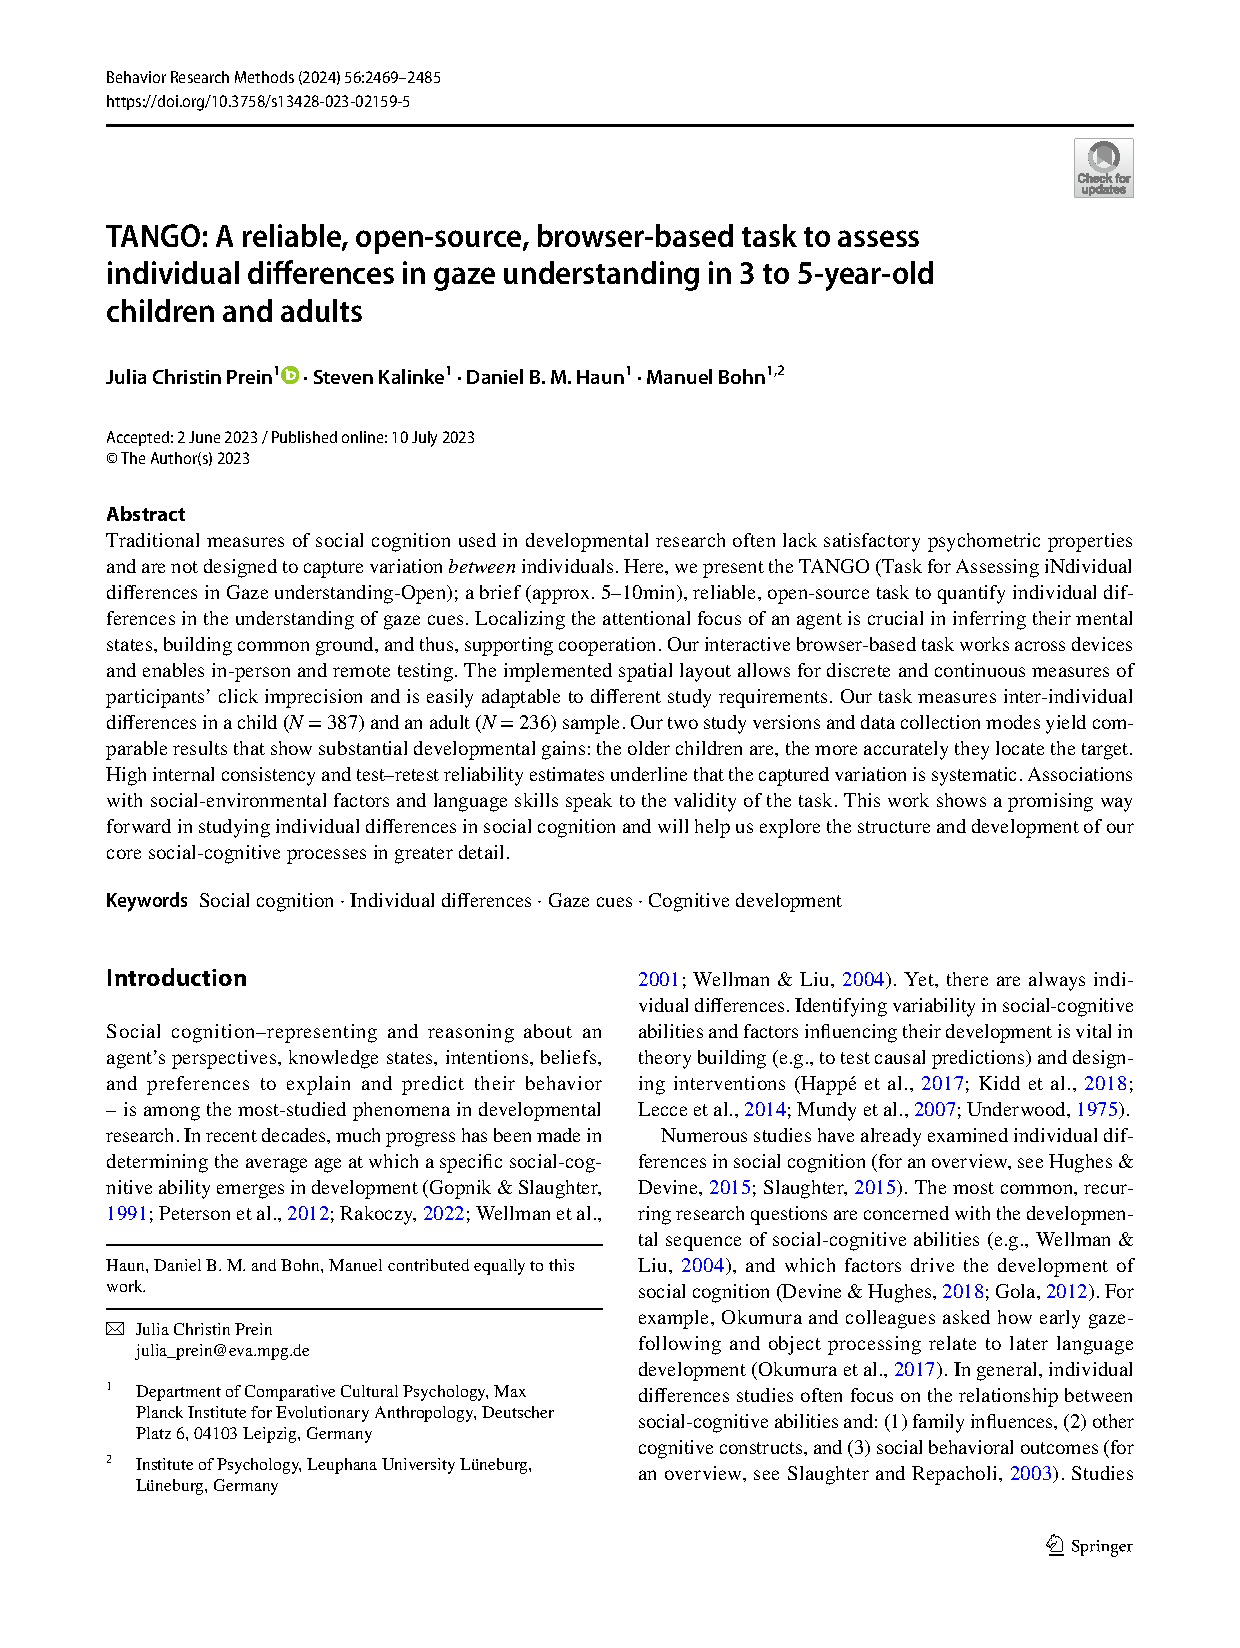
\includepdf[pages={1}, scale=0.85, offset=0 -1cm, pagecommand={}]{../papers/studyI.pdf}
\end{minipage}

\includepdf[pages={2-}, scale=0.85, pagecommand={}]{../papers/studyI.pdf}

\newpage

\section{Study II}\label{studyII}

\begin{minipage}{\textwidth}
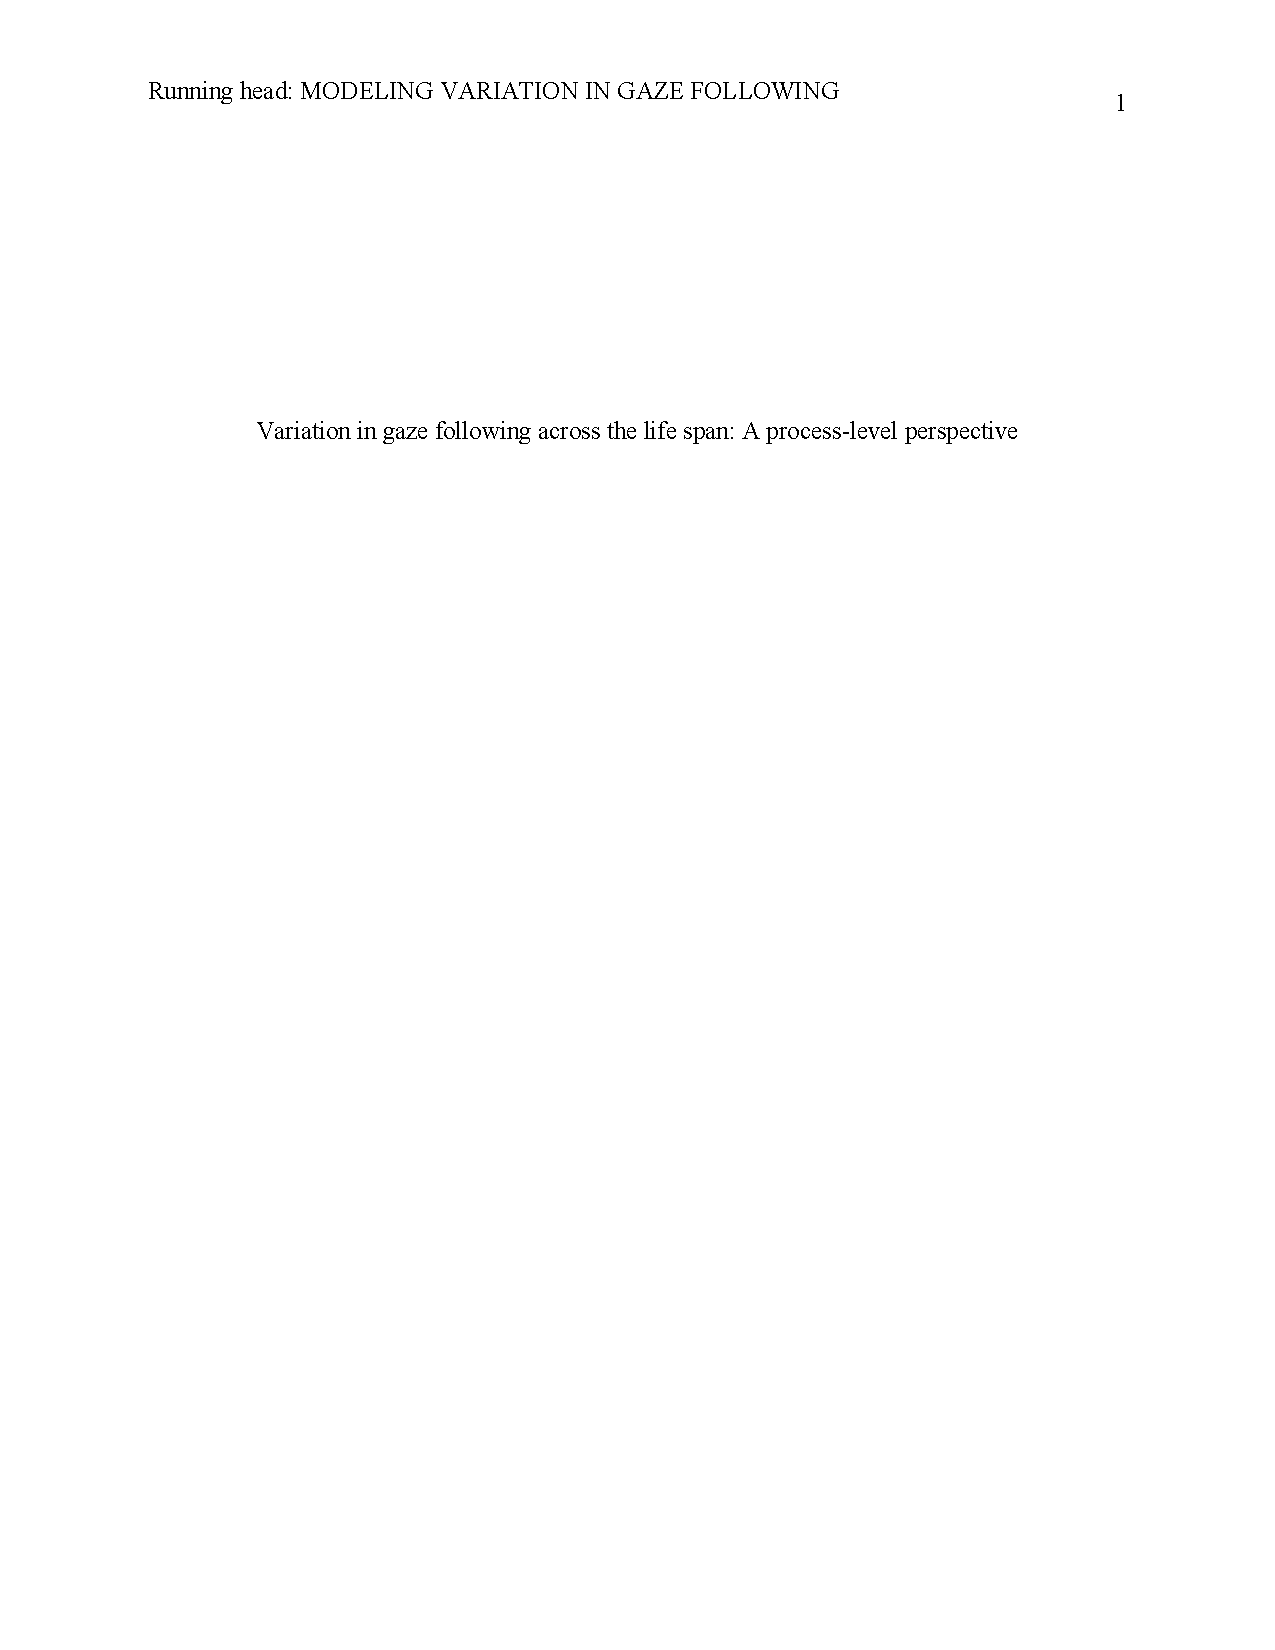
\includepdf[pages={1}, scale=0.85, offset=0 -1cm, pagecommand={}]{../papers/studyII.pdf}
\end{minipage}

\includepdf[pages={2-}, scale=0.85, pagecommand={}]{../papers/studyII.pdf}

\newpage

\section{Study III}\label{studyIII}

\begin{minipage}{\textwidth}
\includepdf[pages={1}, scale=0.85, offset=0 -1cm, pagecommand={}]{../papers/studyIII.pdf}
\end{minipage}

\includepdf[pages={2-}, scale=0.85, pagecommand={}]{../papers/studyIII.pdf}

\newpage

\section{Study IV}\label{studyIV}

\begin{minipage}{\textwidth}

\includepdf[pages={1}, scale=0.85, offset=0 -1cm, pagecommand={}]{../papers/studyIV.pdf}
\end{minipage}


\includepdf[pages={2-}, scale=0.85, pagecommand={}]{../papers/studyIV.pdf}

\chapter{Appendix B --- Further Publications}\label{appendixB}

The following Appendix B contains other publications that were written in the context of the dissertation but not included in the main text, with their respective abstracts.

\section{Action anticipation based on an agent's epistemic state in toddlers and adults}\label{action-anticipation-based-on-an-agents-epistemic-state-in-toddlers-and-adults}

\textbf{Citation:} Schuwerk, T., Kampis, D., Baillargeon, R., Biro, S., Bohn, M., Byers-Heinlein, K., Dörrenberg, S., Fisher, C., Franchin, L., Fulcher, T., Garbisch, I., Geraci, A., Grosse Wiesmann, C., Hamlin, K., Haun, D. B. M., Hepach, R., Hunnius, S., Hyde, D. C., Karman, P., \ldots, Prein, J., \ldots{} Rakoczy, H. (2021). \emph{Action anticipation based on an agent's epistemic state in toddlers and adults. Child Development} (In-Principle Acceptance of Registered Report Stage 1: Study Design). PsyArXiv. \url{https://doi.org/10.31234/osf.io/x4jbm}

\textbf{Abstract:} Do toddlers and adults engage in spontaneous Theory of Mind (ToM)? Evidence from anticipatory looking (AL) studies suggests that they do. But a growing body of failed replication studies raised questions about the paradigm's suitability. In this multi-lab collaboration, we test the robustness of spontaneous ToM measures. We examine whether 18- to 27-month-olds' and adults' anticipatory looks distinguish between two basic forms of an agent's epistemic states: knowledge and ignorance. In toddlers {[}ANTICIPATED n = 520 50\% FEMALE{]} and adults {[}ANTICIPATED n = 408, 50\% FEMALE{]} from diverse ethnic backgrounds, we found {[}SUPPORT/NO SUPPORT{]} for epistemic state-based action anticipation. Future research can probe whether this conclusion extends to more complex kinds of epistemic states, such as true and false beliefs.

\emph{Please note that this abstract was written for the Registered Report and does not entail results yet. Text in square brackets indicates placeholder text to be filled in after data collection.}

\newpage

\section{PREVIC: An adaptive parent report measure of expressive vocabulary in children between 3 and 8 years of age}\label{previc-an-adaptive-parent-report-measure-of-expressive-vocabulary-in-children-between-3-and-8-years-of-age}

\textbf{Citation:} Bohn, M., Prein, J. C., Engicht, J., Haun, D., Gagarina, N., \& Koch, T. (2023). \emph{PREVIC: An adaptive parent report measure of expressive vocabulary in children between 3 and 8 years of age.} PsyArXiv. \url{https://doi.org/10.31234/osf.io/hvncp}

\textbf{Abstract:} Parent report measures have proven to be a valuable research tool to study early language development. Caregivers are given a list of words and are asked which of them their child has already used. However, most available measures are not suited for children beyond infancy, come with substantial licensing costs or lack a clear psychometric foundation. Here we present the PREVIC (Parent Report of Expressive Vocabulary in Children), an open access, high quality vocabulary checklist for German-speaking children between three and eight years of age. The PREVIC was constructed leveraging the advantages of Item Response Theory: we designed a large initial item pool of 379 words and collected data from N = 1190 caregivers of children between three and eight years of age. Based on this data, we computed a range of fit indices for each item (word) and used an automated item selection algorithm to compile a final pool that contains items that a) vary in difficulty and b) fit the Rasch (one-parameter logistic) model. The resulting task is highly reliable and shows convergent validity. The IRT-based construction allowed us to design an adaptive version of the task, which substantially reduces the duration of the task while retaining measurement precision. The task -- including the adaptive version -- was implemented as a website and is freely accessible online (\url{https://ccp-odc.eva.mpg.de/previc-demo/}). The PREVIC fills an important gap in the toolkit of researchers interested in language development and provides an ideal starting point for the development of converging measures in other languages.

\newpage

\section{oREV: An item response theory-based open receptive vocabulary task for 3- to 8-year-old children}\label{orev-an-item-response-theory-based-open-receptive-vocabulary-task-for-3--to-8-year-old-children}

\textbf{Citation:} Bohn, M.*, Prein, J.*, Koch, T., Bee, R. M., Delikaya, B., Haun, D., \& Gagarina, N. (2024). oREV: An item response theory-based open receptive vocabulary task for 3- to 8-year-old children. \emph{Behavior Research Methods, 56}(3), 2595--2605. \url{https://doi.org/10.3758/s13428-023-02169-3}

\textbf{Abstract:} Individual differences in early language abilities are an important predictor of later life outcomes. High-quality, easy-access measures of language abilities are rare, especially in the preschool and primary school years. The present study describes the construction of a new receptive vocabulary task for children between 3 and 8 years of age. The task was implemented as a browser-based web application, allowing for both in-person and remote data collection via the internet. Based on data from N = 581 German-speaking children, we estimated the psychometric properties of each item in a larger initial item pool via item response modeling. We then applied an automated item selection procedure to select an optimal subset of items based on item difficulty and discrimination. The so-constructed task has 22 items and shows excellent psychometric properties with respect to reliability, stability, and convergent and discriminant validity. The construction, implementation, and item selection process described here makes it easy to extend the task or adapt it to different languages. All materials and code are freely accessible to interested researchers. The task can be used via the following website: \url{https://ccp-odc.eva.mpg.de/orev-demo}.

\newpage

\section{Validation of an open source, remote web-based eye-tracking method (WebGazer) for research in early childhood}\label{validation-of-an-open-source-remote-web-based-eye-tracking-method-webgazer-for-research-in-early-childhood}

\textbf{Citation:} Steffan, A., Zimmer, L., Arias-Trejo, N., Bohn, M., Dal Ben, R., Flores-Coronado, M. A., Franchin, L., Garbisch, I., Grosse Wiesmann, C., Hamlin, J. K., Havron, N., Hay, J. F., Hermansen, T. K., Jakobsen, K. V., Kalinke, S., Ko, E.-S., Kulke, L., Mayor, J., Meristo, M., \ldots, Prein, J., \ldots, Schuwerk, T. (2024). Validation of an open source, remote web-based eye-tracking method (WebGazer) for research in early childhood. \emph{Infancy, 29}(1), 31--55. \url{https://doi.org/10.1111/infa.12564}

\textbf{Abstract:} Measuring eye movements remotely via the participant's webcam promises to be an attractive methodological addition to in-person eye-tracking in the lab. However, there is a lack of systematic research comparing remote web-based eye-tracking with in-lab eye-tracking in young children. We report a multi-lab study that compared these two measures in an anticipatory looking task with toddlers using WebGazer.js and jsPsych. Results of our remotely tested sample of 18-27-month-old toddlers (N = 125) revealed that web-based eye-tracking successfully captured goal-based action predictions, although the proportion of the goal-directed anticipatory looking was lower compared to the in-lab sample (N = 70). As expected, attrition rate was substantially higher in the web-based (42\%) than the in-lab sample (10\%). Excluding trials based on visual inspection of the match of time-locked gaze coordinates and the participant's webcam video overlayed on the stimuli was an important preprocessing step to reduce noise in the data. We discuss the use of this remote web-based method in comparison with other current methodological innovations. Our study demonstrates that remote web-based eye-tracking can be a useful tool for testing toddlers, facilitating recruitment of larger and more diverse samples; a caveat to consider is the larger drop-out rate.

\chapter{Appendix C}\label{appendixC}

\chapter{Selbstständigkeitserklärung}\label{selbststaendigkeit}

Julia Christin Prein\\
{[}Straße Hausnummer{]}\\
{[}PLZ Ort{]}\\
{[}Telefon{]}\\
{[}Email{]}\\

Hiermit erkläre ich, dass ich mich noch keiner Doktorprüfung unterzogen oder mich um Zulassung zu einer solchen beworben habe.

Ich versichere, dass die Dissertation {[}TODO: Titel Dissertation{]} in der gegenwärtigen oder einer anderen Fassung noch keiner anderen Hochschule zur Begutachtung vorgelegen hat.

Ich versichere an Eides statt, dass ich die eingereichte Dissertation {[}TODO: Titel Dissertation{]} selbstständig und ohne zulässige fremde Hilfe verfasst habe. Anderer als der von mir angegebenen Hilfsmittel und Schriften habe ich mich nicht bedient. Alle wörtlich oder sinngemäß anderen Schriften entnommenen Stellen habe ich kenntlich gemacht. Über die strafrechtlichen Folgen gemäß § 156 Strafgesetzbuch wurde ich in Kenntnis gesetzt.

~

{[}Ort{]}, {[}Datum{]} ~ ~ {[}Unterschrift{]}

\end{document}
